\chapter{Krav}\label{ch:Krav} %Please start me on a left page :)

I dette afsnit er de opstillede krav for AU2 beskrevet.
Disse krav er opstillet ud fra opgaveformuleringen og ud fra forestillinger om relevante tests af systemet. 
Funktionelle krav er opstillet ud fra Use Cases og ikke-funktionelle krav er opstillet ud fra målbare størrelser.

I figur \ref{fig:use_cases} på side \pageref{fig:use_cases} ses Use Cases for systemet samt en kort beskrivelse af dem. 
De funktionelle krav for systemet er udledt ud fra disse og beskrevet herunder. 
For at se den komplette beskrivelse af kravene for systemet henvises til kapitel \ref{P-ch:kravspecifikation} \nameref{P-ch:kravspecifikation} på side \pageref{P-ch:kravspecifikation} i dokumentationen.

\begin{itemize}
%\begin{packed_item}

\item \textbf{UC1: Aktiver system} sørger for at initialisere systemet ved opstart og beskriver brugerens interaktion med systemet ved opstart.

\item \textbf{UC2: Stream video} initialiserer og vedligeholder streaming af video og beskriver hvad brugeren ser når systemets videostream startes.

\item \textbf{UC3: Overvåg sensorer} indsamler data fra bilens sensorer og analyserer om en undvigelsesmanøvre er nødvendig for at bilen ikke kører ind i noget.

\item \textbf{UC4: Undvig forhindring} styrer automatisk bilen udenom en forhindring ved at manipulere bilens styrtøj og motor.

\item \textbf{UC5: Kør bil frem/tilbage} beskriver brugerens interaktion med systemet når vedkommende ønsker at køre fremad eller at bakke. 
Det beskrives ligeledes hvordan AKS overtager kontrol over bilen for at undvige forhindringer.

\item \textbf{UC6: Drej bil til højre/venstre} beskriver brugerens interaktion med systemet når brugeren ønsker at få bilen til at dreje til enten højre eller venstre. Beskriver ydermere antikollisionssystemets overtagelse af brugerkontrollen.

\item \textbf{UC7: Brems bil} beskriver hvordan bilen bremses både af bruger og af antikollissionssystemet.

\item \textbf{UC8: Konfigurer IP-adresse} beskriver hvordan brugeren indstiller IP-adressen for bilen i PC softwaren

\item \textbf{UC9: Tænd/sluk AKS} beskriver hvordan brugeren slår antikollissionssystemet fra eller til.

\item \textbf{UC10: Indstil makshastighed} beskriver hvordan brugeren indstiller en ny makshastighed for bilen.

\item \textbf{UC11: Kalibrer styrtøj} beskriver hvordan brugeren kalibrer styrtøjet, så bilen kører ligeud.

\item \textbf{UC12: Afbryd system} beskriver hvad der sker, når systemet afbrydes eller lukkes ned af brugeren.

%\end{packed_item}
\end{itemize}

Bilen skal kunne køre frem og tilbage, dreje og give brugeren mulighed for at begrænse makshastigheden af bilen. 
Styringen af bilen skal foregå med en Xbox-360 Controller fra en PC via et Wi-Fi netværk til bilens Raspberry Pi.
Bilen skal selv via afstandssensorerne kunne identificere en forhindring forude, og hvis AKS er aktiveret skal dette styre bilen udenom forhindringen eller bremse bilen.
Brugeren skal ydermere via den grafiske brugerflade på PC'en kunne se et live video feed fra et kamera ombord på bilen.
Brugeren bør kunne aktivere og deaktivere AKS ved hjælp af PC softwaren.
Bilen bør være udstyret med bremselys, som lyser ved bremsning.

De ikke-funktionelle krav findes i afsnit \ref{P-sec:ikke-funktionelle_krav} \nameref{P-sec:ikke-funktionelle_krav} på side \pageref{P-sec:ikke-funktionelle_krav} i dokumentationen.

\clearpage

\begin{figure}[h]
\centering
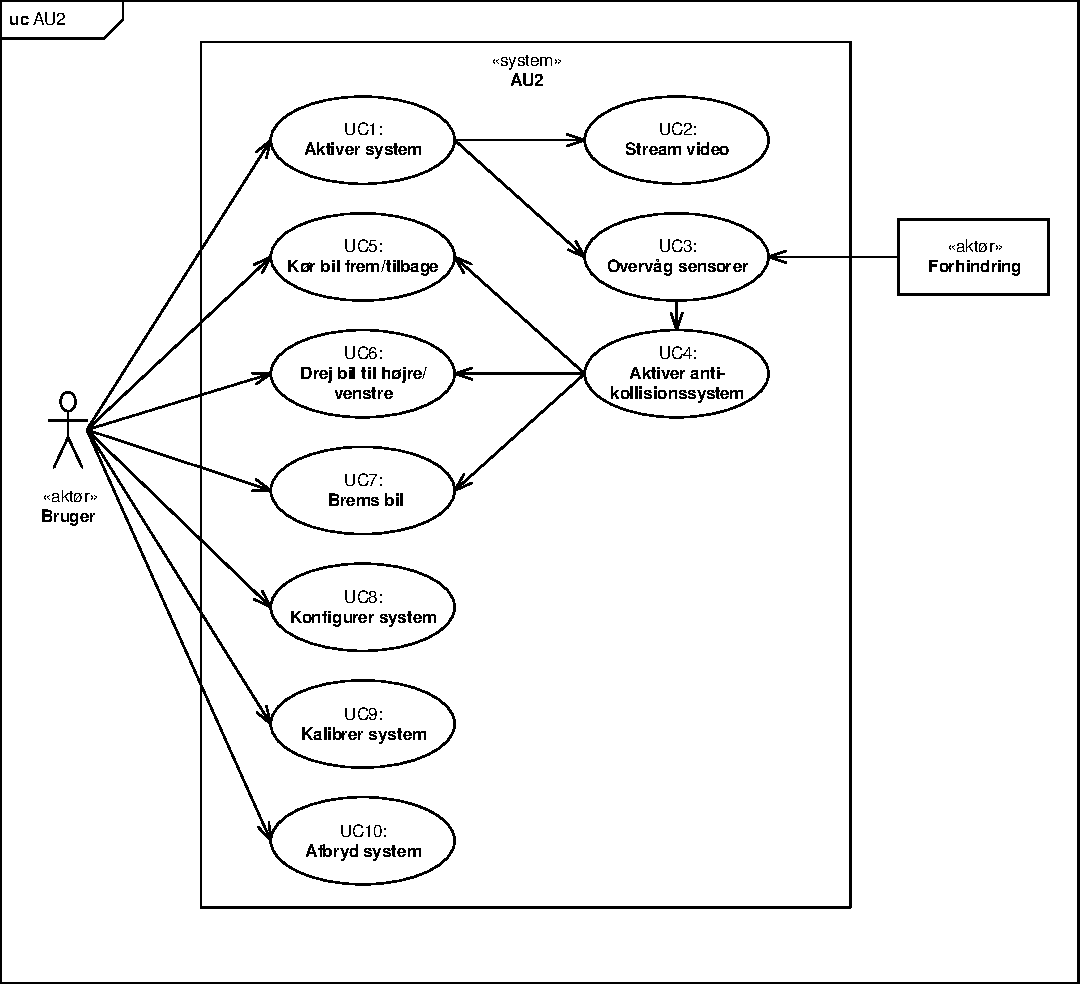
\includegraphics[width=\textwidth]{../fig/diagrammer/uc_au2}
\caption{Use Cases for AU2.}
\label{fig:use_cases}
\end{figure}